\documentclass[a4paper, fontsize=11pt]{article}

\usepackage{amsmath,amsfonts,amsthm} % Math packages
\usepackage[english]{babel} % English language/hyphenation
%\usepackage{hyperref}
\usepackage{listings}
\usepackage{color}
\usepackage{verbatim}
\usepackage{graphicx}
\usepackage{float}
\usepackage{pgfplotstable, booktabs, mathpazo}


\usepackage[colorlinks=true,linkcolor=black,urlcolor=blue,
citecolor=blue]{hyperref}

%\bibliographystyle{ieeetr}
\bibliographystyle{apalike}

\definecolor{dkgreen}{rgb}{0,0.6,0}
\definecolor{gray}{rgb}{0.5,0.5,0.5}
\definecolor{mauve}{rgb}{0.58,0,0.82}


\lstset{frame=tb,
  language=C++,
  aboveskip=3mm,
  belowskip=3mm,
  showstringspaces=false,
  columns=flexible,
  basicstyle={\small\ttfamily},
  numbers=none,
  numberstyle=\tiny\color{gray},
  keywordstyle=\color{blue},
  commentstyle=\color{dkgreen},
  stringstyle=\color{mauve},
  breaklines=true,
  breakatwhitespace=true,
  tabsize=3
}

\pgfplotstableset{
    every head row/.style={before row=\toprule,after row=\midrule},
    every last row/.style={after row=\bottomrule}
}

\begin{document}

\title{Project 3 FYS4150 \\ Ordinary differential equations}
\author{Audun Tahina Reitan and Marius Holm}

%----------------------------------------------------------------------------------------
%	PROBLEM 1
%----------------------------------------------------------------------------------------
\maketitle


\section{Abstract}
We give a brief introduction to differential equations and how we can discretize such equations in order to solve them using computer algorithms. 

\paragraph{}
More of our results can be found in the GitHub repository linked in the implementation section. 

\section{Introduction}
In this project we'll develop code for simulating the solar system, using the Verlet algorithm for solving coupled ordinary differential equations. For this project we will focus on the use of classes in our code, which makes it a lot easier to reuse larger parts of our code for problems of similar character. In our case of the solar system we can create a class describing a planet, a moon, or some other astronomical body which we want to include in our solar system.


\paragraph{}
In order to test that our algorithm works, we start by looking at a simple hypothetical system consisting of only the Earth orbiting the Sun. We then investigate the stability of our algorithm and plot the position of the Earth orbiting the Sun. Furthermore we consider the initial velocity needed for the planet to escape the gravity of the Sun. Then we'll consider a three-body system consisting of the Earth, the Sun, and Jupiter. We then expand our three-body model to the entire solar system including Pluto. In the final part of our project we look at the perihelion precession of Mercury.



\section{Methods}


\subsection{Differential equations}
The order of an ordinary differential equation (ODE) is given by the highest order of derivative found in the left-hand side of the equation. A first order differential equation is typically of the form 

\begin{equation}
\dfrac{dy}{dt} = f\big(t,\dfrac{dy}{dt},y\big)
\end{equation}

where $f$ is an arbitrary function. A well known second order differential equation is Newton's second law 

\begin{equation}
m \dfrac{d^2 x}{dt^2}=-kx
\end{equation}

where $k$ is the force constant. All ODE's depend on one variable only, compared to partial differential equations which can depend on several variables. PDE's are widely used, but won't be of any concern in this project.


\subsection{Newton's law of gravitation}
The first part of our project we take a look at a simplified solar system consisting of the Sun and the Earth. Newton's law of gravitation then takes the following form:

\begin{equation}
F_{G} = \dfrac{G M_{\odot}M_{Earth}}{r^2},
\end{equation}

where $M_{\odot}$ is the mass of the Sun and $M_{Earth}$ is the mass of the Earth. $G$ is the gravitational constant and $r$ is the distance between the Earth and the Sun.

\paragraph{}
We assume that the orbit of the Earth around the sun is co-planar, and we let this be the $xy$-plane. We can then use Newton's second law of motion which gives us two differential equations, one for each coordinate.

\begin{equation}
\dfrac{d^2x}{dt^2}=\dfrac{F_{G,x}}{M_{Earth}},
\end{equation}

and 

\begin{equation}
\dfrac{d^2y}{dt^2}=\dfrac{F_{G,y}}{M_{Earth}},
\end{equation}

where $F_{G,x}$ and $F_{G,y}$ are the $x$ and $y$ components of the gravitational force.


\subsection{Useful constants}
During our project we will use astronomical units (AU) as a measure of length. 1 AU is defined as the average distance between the Sun and the Earth, that is 1 AU $= 1.5 \times 10^{11}$ m. The mass of the Sun is $M_{\text{sun}}=M_{\odot}=2 \times 10^{30}$ kg. We will also need the mass of the planets we include in our code, which are given in table \ref{PlanetMass}. In our code we have defined the unit mass to be equal to $M_{\odot}$, i.e. $M_{\odot}=1$. We therefore also present the planetary masses given in the unit $M_{\odot}$.

\begin{table}[H]
\begin{center}
\caption{Mass and distance from the Sun for each planet in our solar system.}
\begin{tabular}{l l l c}
\toprule
Planet & Mass in kg & Mass in unit $M_{\text{Sun}}$ & Distance to sun in AU \\ \midrule
Earth    &    $M_{\text{Earth}}=6 \times 10^{24} $ kg & $3.04 \times 10^{-6}$ &    1 AU\\
Jupiter    &    $M_{\text{Jupiter}}=1.9 \times 10^{27} $ kg & $9.54 \times 10^{-4}$ &   5.20 AU\\
Mars    &    $M_{\text{Mars}}=6.6 \times 10^{23} $ kg &  $3.23 \times 10^{-7}$  & 1.52 AU\\
Venus    &    $M_{\text{Venus}}=4.9 \times 10^{24} $ kg &  $2.45 \times 10^{-6}$  &  0.72 AU\\
Saturn    &    $M_{\text{Saturn}}=5.5 \times 10^{26} $ kg &  $2.86 \times 10^{-4}$  &  9.54 AU\\
Mercury    &    $M_{\text{Mercury}}=3.3 \times 10^{23} $ kg &  $1.66 \times 10^{-7}$ &   0.39 AU\\
Uranus    &    $M_{\text{Uranus}}=8.8 \times 10^{25} $ kg &  $4.37 \times 10^{-5}$ &   19.19 AU\\
Neptune    &    $M_{\text{Neptune}}=1.03 \times 10^{26} $ kg &  $5.15 \times 10^{-5}$  & 30.06 AU\\
Pluto    &    $M_{\text{Pluto}}=1.31 \times 10^{22} $ kg &  $7.40 \times 10^{-9}$ &   39.53 AU\\
\bottomrule
\end{tabular}
\label{PlanetMass}
\end{center}
\end{table}

We include Pluto, even though it is technically not regarded as a planet anymore. 

\subsection{Discretizing differential equations}
We assume that Earth's orbit is circular around the Sun. For circular motion we have

\begin{equation}
F_{G} = \dfrac{M_{\text{Earth}}v^2}{r}=\dfrac{GM_{\odot} M_{\text{Earth}}}{r^2},
\end{equation}

where $v$ is Earth's velocity. By simple algebraic manipulation we find the relationship

\begin{equation}
v^2 r = G M_{\odot}=4 \pi^2 \: \text{AU}^3/\text{yr}^2
\end{equation}

By defining $M_{\odot} = 1$ we have $G=4\pi^2 \: \text{AU}^3/\text{yr}^2$.



\subsubsection{Euler's forward algorithm}
Suppose we have an initial function value $y(t_{0})=y(t=t_{0})$ for a function $y(t)$. The function is defined in the well-behaved domain $[a, b]$. By splitting the domain into $N$ sub intervals we find the step size $h$ as

\begin{equation}
h=\dfrac{b-a}{N}.
\end{equation}

Using the step size, $h$, and the derivative of $y$ we can find an expression for the function at the next time step as $y_{1}=y(t_{1}=t_{0}+h)$. We can generalize this method which gives us a general procedure for finding the step $y_{i+1}$ in terms of the previous time step.

\begin{equation}
y_{i+1}=y(t=t_{i}+h)=y(t_{i})+h \Delta \big(t_{i},y_{i}(t_{i}) \big) + O(h^{p+1}),
\end{equation}

where $O(h^{p+1})$ represents the truncation error. Using Taylor expansion we find 

\begin{equation}
\Delta \big(t_{i}, y_{i}(t_{i}) \big) =(y'(t_{i}) + \cdots + y^{(p)}(t_{i})\dfrac{h^{p-1}}{p!}
\end{equation}

By defining $y'(t_{i})=f(t_{i}, y_{i})$ and truncating $\Delta$ at the first derivative, we have 

\begin{equation}
y_{i+1}=y_{i} + h f(t_{i},y_{i}) + O(h^2)
\end{equation}

which combined with $t_{i+1}=t_{i}+h$ gives us Euler's forward algorithm. \cite{H-Jensen}

\subsubsection{Euler's method specific}
Introducing $x = r \cos \theta$, $y=r \sin \theta$ and $r=\sqrt{x^2+y^2}$ we can rewrite 

\begin{equation}
F_{G,x}=-\dfrac{GM_{\odot} M_{\text{Earth}}}{r^2} \cos \theta = - \dfrac{G M_{\odot} M_{\text{Earth}}}{r^3} x
\end{equation}

Similarly for y-direction we get

\begin{equation}
F_{G,y}=-\dfrac{GM_{\odot} M_{\text{Earth}}}{r^2} \sin \theta = - \dfrac{G M_{\odot} M_{\text{Earth}}}{r^3} y
\end{equation}
 

\paragraph{}
This gives us the four coupled differential equations 

\begin{align}
\dfrac{dv_{x}}{dt}=-\dfrac{G M_{\odot}}{r^3}x, \\
\dfrac{dx}{dt} = v_{x}, \\
\dfrac{dv_{y}}{dt}=-\dfrac{G M_{\odot}}{r^3}y, \\
\dfrac{dy}{dt} = v_{y},
\end{align}


The four equations can then be discretized using Euler's forward algorithm, and we find the four discretized equations as

\begin{equation}
x_{i+1} = x_{i} + h v_{x,i},
\end{equation}

\begin{equation}
v_{x,i+1} = v_{x,i} - h \dfrac{4 \pi^2}{r_{i}^3}x_{i},
\end{equation}


\begin{equation}
y_{i+1} = y_{i} + h v_{y,i},
\end{equation}

\begin{equation}
v_{y,i+1} = v_{y,i} - h \dfrac{4 \pi^2}{r_{i}^3}y_{i}.
\end{equation}

When adding more planets these equations have to be modified. We will show how this is done in the case of adding Jupiter to our system. The additional gravitational force on Earth from Jupiter in the x-direction is 

\begin{equation}
F_{x}^{EJ} = -\dfrac{G M_{J} M_{E}}{r^3_{EJ}}(x_{E} - x_{J}),
\end{equation}

where $M_{E}$ is the mass of the Earth, $M_{J}$ is the mass of Jupiter, and 

\begin{equation}
r_{EJ}=\sqrt{(x_{E}-x_{J})^2 + (y_{E}- y_{J})^2 }.
\end{equation}

$x_{E}$ and $y_{E}$ are the $x$ and $y$ coordinates of Earth, while $x_{J}$ and $y_{J}$ are the $x$ and $y$ coordinates of Jupiter. Thus the velocity of Earth changes as

\begin{equation}
\dfrac{dv_{x}^{E}}{dt}=-\dfrac{G M_{\odot}}{r^3}x_{E} - \dfrac{G M_{J}}{r_{EJ}^3}(x_{E}-x_{J})
\end{equation}

By using $G M_{J} = G M_{\odot} \Big(\dfrac{M_{J}}{M_{\odot}}\Big)=4\pi^2 \dfrac{M_{J}}{M_{\odot}}$ we can rewrite the equation as

\begin{equation}
\dfrac{dv_{x}^{E}}{dt}=-\dfrac{4\pi^2}{r^3}x_{E} - \dfrac{4\pi^2 \frac{M_{J}}{M_{\odot}} }{r_{EJ}^3}(x_{E}-x_{J}).
\end{equation}

Similarly for the y-direction we get

\begin{equation}
\dfrac{dv_{y}^{E}}{dt}=-\dfrac{4\pi^2}{r^3}y_{E} - \dfrac{4\pi^2 \frac{M_{J}}{M_{\odot}} }{r_{EJ}^3}(y_{E}-y_{J}).
\end{equation}

These equations also apply to Jupiter, and very similar equations apply to the other possible planets we might add to our system.

\subsubsection{Velocity Verlet method}



The final equations for position and velocity are then given by

\begin{equation}
x_{i+1} = x_{i} + h v_{i} + \dfrac{h^2}{2} v_{i}^{(1)} + O(h^3),
\end{equation}

and 

\begin{equation}
v_{i+1} = v_{i} + \dfrac{h}{2} \Big( v_{i+1}^{(1)} +v_{i}^{(1)} \Big) + O(h^3).
\end{equation}



\subsection{Implementation}

.\cite{H-Jensen} 


\paragraph{}
All our code, calculations, and plots used can be found in \href{https://github.com/auduntre/FYS4150/tree/master/Project%203}{Auduns GitHub repository}.

\section{Results}
\subsection{Preservation of dot product}

\begin{figure}[H]
\centering
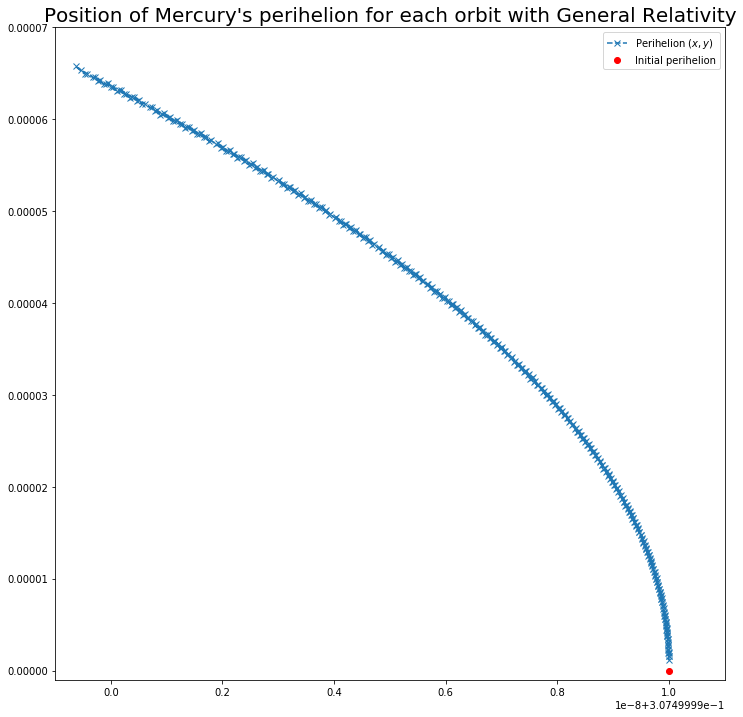
\includegraphics[scale=0.5]{plots/GeneralRelativityMercury}
\caption{General relativity Mercury.}
\label{GRMercury}
\end{figure}


\begin{figure}[H]
\centering
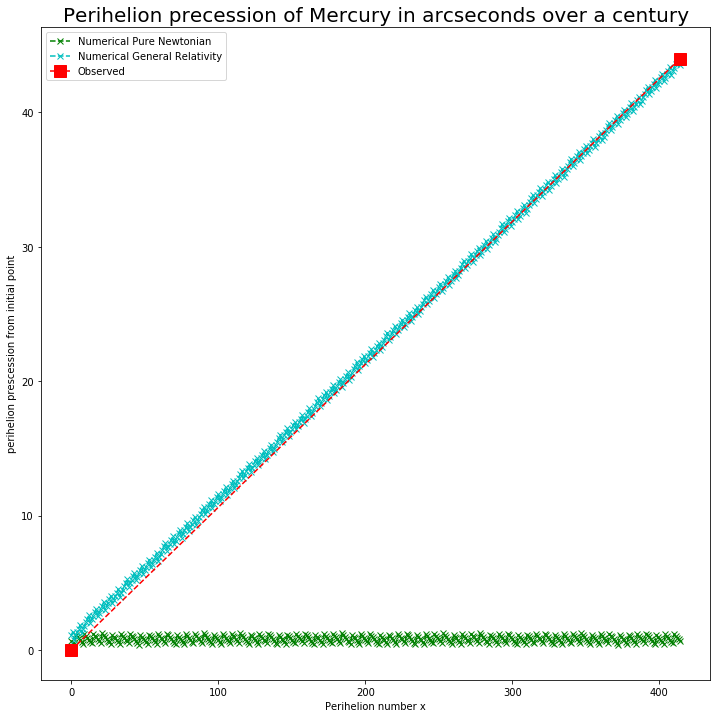
\includegraphics[scale=0.5]{plots/PerihelionPrecessionMercury}
\caption{Perihelion precession of Mercury.}
\label{PerihelionMercury}
\end{figure}

\begin{figure}[H]
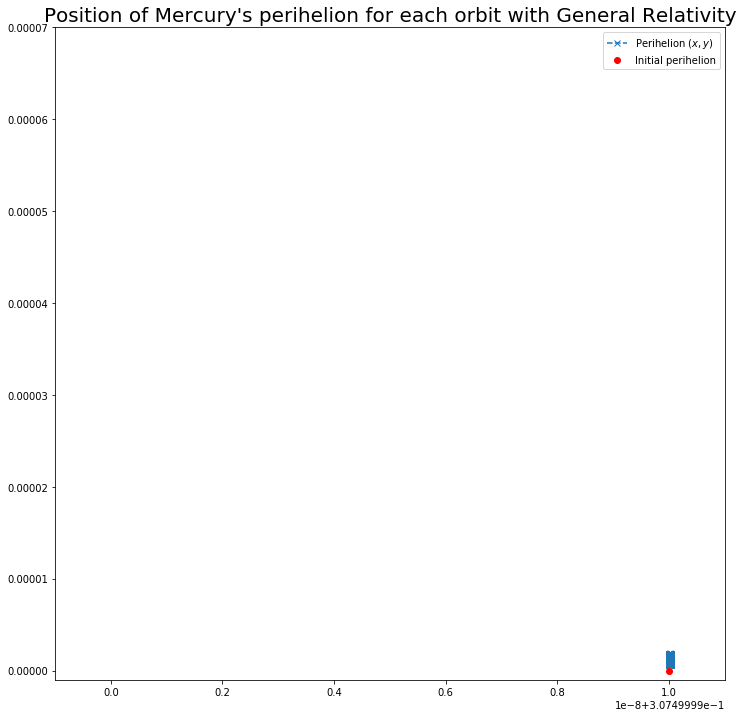
\includegraphics[scale=0.5]{plots/NewtonianMercury}
\caption{Newtonian Mercury.}
\label{fig:NewtonianMercury}
\end{figure}

\paragraph{}
Testing Anders' code for automatic inclusion of data to table.
\begin{table}[h!tb]
    \centering
    \caption{The greatest table.}
    \pgfplotstabletypeset[sci]{error.dat}
\end{table}



\subsection{Eigenvalues of one electron in the harmonic oscillator}







\section{Discussion}
\subsection{Jacobi method}

 




\bibliography{references}
\end{document}